% Modelo de despliegue (ADR-0001): la computadora del centro de acopio funciona
% como servidor local y los demás dispositivos se conectan por la red local.
\documentclass[tikz,border=0pt]{standalone}
% Estilo común de los diagramas de los ADR.
\usepackage[T1]{fontenc}
\usepackage[utf8]{inputenc}
\usepackage[sfdefault]{FiraSans}
\usepackage{fontawesome5}
\usetikzlibrary{positioning,backgrounds,fit,arrows.meta,calc}

% Capa para los recuadros de zona: encima del fondo blanco y debajo de los equipos.
\pgfdeclarelayer{zonas}
\pgfsetlayers{background,zonas,main}

\definecolor{texto}{HTML}{262626}
\definecolor{azul}{HTML}{1F4E79}
\definecolor{naranja}{HTML}{C55A11}
\definecolor{gris}{HTML}{8C8C8C}

\tikzset{
  % Se aplica en cada tikzpicture: fondo blanco para que se lea en modo oscuro.
  diagrama/.style={
    font=\small, color=texto,
    background rectangle/.style={fill=white},
    show background rectangle, inner frame sep=14pt,
  },
  % Dispositivo con icono, título y descripción opcional.
  equipo/.style={
    draw=#1, fill=#1!10, line width=0.9pt, rounded corners=5pt,
    align=center, font=\footnotesize, inner sep=6pt, minimum width=3.1cm, minimum height=1.9cm,
  },
  equipo/.default=azul,
  % Recuadro que agrupa los equipos de un centro o una etapa.
  zona/.style={
    draw=#1, line width=0.8pt, rounded corners=8pt, inner sep=12pt,
  },
  zona/.default=gris,
  titulozona/.style={
    anchor=south west, font=\small\bfseries, text=#1, inner sep=3pt,
  },
  titulozona/.default=gris,
  enlace/.style={Latex-Latex, line width=0.9pt, draw=azul},
  copia/.style={-Latex, line width=1.1pt, draw=naranja},
  etiqueta/.style={font=\footnotesize, fill=white, inner sep=2pt, align=center},
  nota/.style={
    draw=#1, fill=#1!6, line width=0.7pt, rounded corners=4pt,
    font=\footnotesize, align=center, inner sep=5pt,
  },
  nota/.default=gris,
}

% \equipotexto{icono}{título}{descripción}
% La descripción usa el tamaño de letra del nodo, porque TikZ no conserva un cambio
% de tamaño después de \\ ni admite \\ dentro de un grupo.
\newcommand{\equipotexto}[3]{{\Large #1}\\[3pt]{\small\bfseries #2}\\[1pt]#3}


\begin{document}
\begin{tikzpicture}[diagrama, node distance=1.2cm and 0.6cm]

  \node[equipo, minimum width=4.4cm] (servidor)
    {\equipotexto{\faLaptop}{Servidor local}{Computadora del centro\\Los datos se guardan en ella}};

  \node[equipo, below left=1.9cm and 0.4cm of servidor] (vol1)
    {\equipotexto{\faMobile*}{Voluntario}{Teléfono, navegador}};
  \node[equipo, below=1.9cm of servidor] (vol2)
    {\equipotexto{\faMobile*}{Voluntario}{Teléfono, navegador}};
  \node[equipo, below right=1.9cm and 0.4cm of servidor] (coord)
    {\equipotexto{\faMobile*\,\faLaptop}{Coordinador}{Teléfono o computadora,\\navegador}};

  \draw[enlace] (servidor.south) -- (vol1.north);
  \draw[enlace] (servidor.south) -- (vol2.north);
  \draw[enlace] (servidor.south) -- (coord.north);
  \node[etiqueta, text=azul] at ($(servidor.south)!0.5!(vol2.north)$)
    {\faWifi\ Red local (Wi-Fi), sin internet};

  \begin{pgfonlayer}{zonas}
    \node[zona=azul, fit=(servidor) (vol1) (vol2) (coord)] (centro) {};
  \end{pgfonlayer}
  \node[titulozona=azul] at (centro.north west) {Centro de acopio};

\end{tikzpicture}
\end{document}
